
\documentclass[article, 9pt]{extarticle}
\usepackage{amsmath}
\usepackage{lineno,hyperref}
\usepackage[table,x11names,dvipsnames,table]{xcolor}
\usepackage{authblk}
\usepackage{subcaption,booktabs}
\usepackage{graphicx}
\usepackage{multirow}
\usepackage[nolist,nohyperlinks]{acronym}
\usepackage[superscript]{cite}
\usepackage{tabularx}
\usepackage{float}
\usepackage[group-separator={,}]{siunitx}
\usepackage{geometry}
 \geometry{
 a4paper,
 papersize={210mm,279mm},
 left=9mm,
 top=15mm,
 marginpar=3.53mm,
 textheight=238.4mm,
 right=9mm,
 }


\setlength{\columnsep}{6.54mm}

%\linenumbers %%% Turn on line numbers here

\renewcommand{\familydefault}{\sfdefault}

\captionsetup[figure]{labelfont=bf,textfont=normalfont}
\captionsetup[subfigure]{labelfont=bf,textfont=normalfont}


%%%% comment out the below for the other title option
\makeatletter
\def\@maketitle{
\raggedright
\newpage
  \noindent
  \vspace{0cm}
  \let \footnote \thanks
    {\hskip -0.4em \huge \textbf{{\@title}} \par}
    \vskip 1.5em
    {\large
      \lineskip .5em
      \begin{tabular}[t]{l}
      \raggedright
        \@author
      \end{tabular}\par}
    \vskip 1em
  \par
  \vskip 1.5em
  }
\makeatother





\begin{document}


\title{Conducting Microchip Research: An Analyzation of NVIDIA Corporation Stocks}

\author[1, 2]{Written by Neya Sathiya}


\setcounter{Maxaffil}{0}
\renewcommand\Affilfont{\itshape\small}

\date{}  
\maketitle

\section{Introduction}

With there being well over 450 semiconductor companies as of 2024, the top 10 corporations have especially stood out with their market capitalization ranging from billions, to even trillions of dollars. The number one semiconductor company that has broke records in its revenue and surpassed stocks across all industries is none other than NVIDIA Corporation. NVIDIA is primarily the largest manufacturers for graphics processing units (GPUs) and other advanced microchips. These products have always been
essential for other large companies, leading us to wonder: what truly sets NVIDIA apart?

\section{The Semiconductor Companies of the World}

\begin{minipage}[t]{0.4\textwidth}

\subsection{Top 10 Companies}

    \begin{enumerate}
        \item Nvidia Corporation (US)
        \item Broadcom Inc. (US)
        \item Taiwan Semiconductor Manufacturing Company Limited (Taiwan)
        \item Advanced Micro Devices, Inc. (US)
        \item Intel Corporation (US)
        \item Qualcomm Incorporated (US)
        \item Texas Instruments Incorporated (US)
        \item Analog Devices, Inc. (US)
        \item Micron Technology, Inc. (US)
        \item SK hynix, Inc. (South Korea)
    \end{enumerate}
\end{minipage}
\hfill
\begin{minipage}[t]{0.6\textwidth}
\centering
    \begin{figure}[H]
        \centering
        \includegraphics[width=\linewidth]{bar_graph.png}
    \end{figure}
\end{minipage}




\subsection{Examining Market Capitalization}

To start off, NVIDIA is a noticeably worth more than the other companies on this graph. In fact, its market capitalization is more than twice of the second largest semiconductor industry, demonstrating its evident superiority in the stock market. Following NVIDIA is Broadcom Incorporations and Taiwan Semiconductor Manufacturing Company Limited, which are both still considered as some of the largest tech companies. The next 7 companies are still extremely successful in a competitive market, but haven't shown the significant growth and spike that NVIDIA has.

\section{NVIDIA's Recent Success}

Although NVIDIA was officially released on January 22, 1999, the software company primarily took off from 2022 to 2024. The reason as to why it is so valuable is because its drivers allows for a sense of communication between the computer and the GPU in the system, ensuring that the hardware is utilizing the appropriate, updated software. This AI-applicable interface became particularly crucial during semiconductor shortages, leading to a surge in demand. 

\subsection{NVIDIA Stocks of May 2024}

\begin{figure}[H]
        \centering
        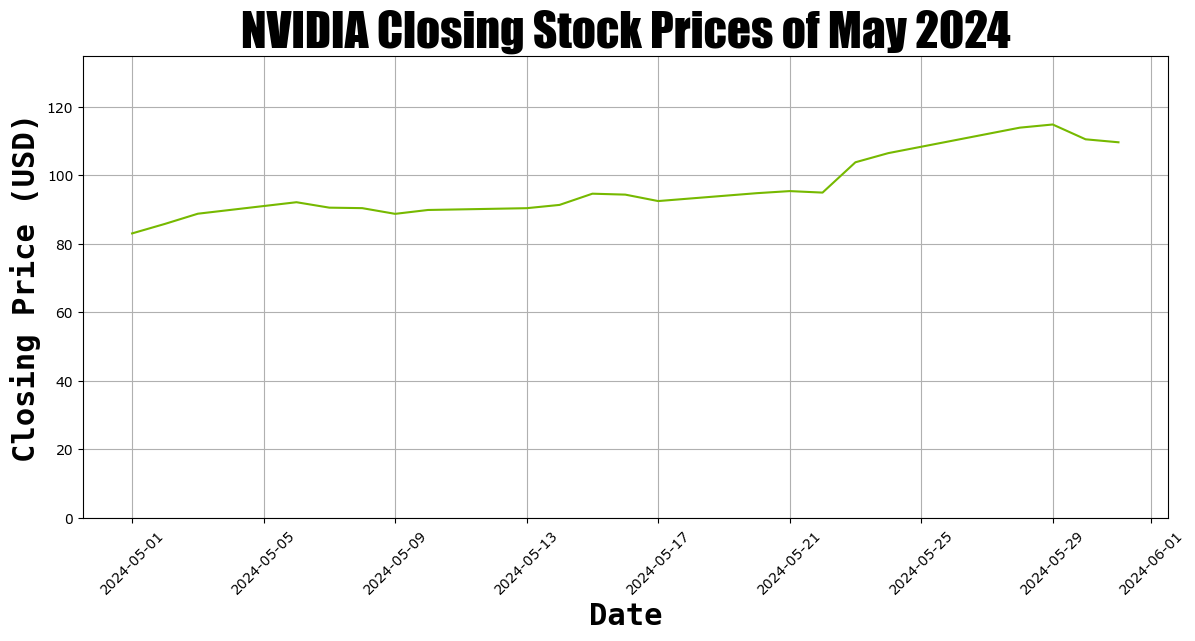
\includegraphics[width=\linewidth]{line_graph_may.png}
    \end{figure}


\begin{figure}[H]
        \centering
        \includegraphics[width=0.7\linewidth]{ohlc_may.png}
    \end{figure}


\section{25 Years of NVIDIA Stocks: 1999-2024}

\begin{figure}[H]
        \centering
        \includegraphics[width=\linewidth]{line_graph_1999.png}
    \end{figure}


\begin{figure}[H]
        \centering
        \includegraphics[width=0.65\linewidth]{ohlc_1999.png}
    \end{figure}


\end{document}